
With this definition we conclude the presentation of the three semantic variants of $\HS$.
In the next sections  we will compare the expressiveness of the logics $\HS_{\stat}$, $\HS_{\LinearPast}$, $\HS_{\LinearTime}$, $\LTL$, $\CTL$, and $\CTLStar$ when interpreted over finite Kripke structures.

Given two logics $L_1$ and $L_2$, and two formulas $\varphi_1\in L_1$ and $\varphi_2\in L_2$, we say that   $\varphi_1$ in $L_1$ is \emph{equivalent} to  $\varphi_2$ in $L_2$ if, for every finite Kripke structure   $\Ku$, 
$\Ku$ is a model of $\varphi_1$ in $L_1$ if and only if $\Ku$ is a model of $\varphi_2$ in $L_2$. 
%When comparing the expressive power of two logics $L_1$ and $L_2$, 
We say that \emph{$L_2$ is subsumed by $L_1$}, denoted as $L_1\geq L_2$, if for each formula $\varphi_2\in L_2$, there exists a formula $\varphi_1\in L_1$ such that $\varphi_1$ in $L_1$ is equivalent to $\varphi_2$
in $L_2$. Moreover, $L_1$ is \emph{as expressive as} $L_2$ (or, $L_1$  and $L_2$ have \emph{the same expressive power}), written $L_1\equiv L_2$, if both $L_1\geq L_2$ and $L_2\geq L_1$. We say that  $L_1$ is \emph{(strictly) more expressive than} $L_2$ if $L_1\geq L_2$ and $L_2\not\geq L_1$. Finally, $L_1$ and $L_2$ are \emph{expressively incomparable} if both $L_1\not\geq L_2$ and $L_2\not\geq L_1$.

\subsection{An example: a vending machine}\label{subs:vendingMach}
In this section, we give an example highlighting the differences among the $\HS$ semantic variants $\HS_\stat$, $\HS_\LinearPast$, and $\HS_\LinearTime$.

\begin{figure}[tp]
\centering
\resizebox{\textwidth}{!}{
\begin{tikzpicture}[->,>=stealth',shorten >=1pt,auto,node distance=2.8cm,semithick]
  \tikzstyle{every state}=[inner sep=1pt, outer sep=0pt, minimum size = 40pt]

  \node[accepting,state] (A0)                    {$\stackrel{s_0}{p_\text{\$=0}}$};
  \node[state]         (B2) [below of=A0] {$\stackrel{s_2}{p_\text{\$=2}}$};
  \node[state]         (B1) [left of=B2] {$\stackrel{s_1}{p_\text{\$=1}}$};
  \node[state]         (B05) [right of=B2] {$\stackrel{s_3}{p_\text{\$=0.50}}$};
  \node[state]         (C1) [below of=B1] {$\stackrel{s_4}{p_\text{candy}}$};
  \node[state]         (C2) [below of=B2] {$\stackrel{s_5}{p_\text{hotdog}}$};
  \node[state]         (C05) [below of=B05] {$\stackrel{s_6}{p_\text{water}}$};
  \node[state]         (D) [below of=C2] {$\stackrel{s_7}{p_\text{change}}$};
  
  \node[state]         (M1) [right of=C05] {$\stackrel{s_8}{p_\text{maint}}$};
  \node[state]         (M2) [right of=B05] {$\stackrel{s_9}{p_\text{maint\_end}}$};
  
  \path (A0) edge  [swap]  node {ins\_\$2} (B2)
            edge  [bend right,swap]  node {ins\_\$1} (B1)
            edge  [bend left,swap]  node {ins\_\$0.50} (B05)
        (B2) edge  [near start]  node {sel} (C2)
             edge  [near end]  node {sel} (C1)
             edge   node {sel} (C05)
        (B1) edge   node {sel} (C1)
             edge  [very near start]  node {sel} (C05)
        (B05) edge  [near end]  node {sel} (C05)
        (C1) edge   [bend right,very near start]  node {dispensed} (D)
        (C2) edge  [swap]  node {dispensed} (D)
        (C05) edge  [bend left,swap]  node {dispensed} (D)
        (D) edge   [bend right,swap]  node {change\_given} (M1)
        (D) edge   [out=200,in=160,looseness=1.7]  node {change\_given} (A0)
        (M1) edge  [near end]  node {maint\_ongoing} (M2)
        (M2) edge [bend left] node {maint\_failed} (M1)
        (M2) edge   [bend right,swap]  node {maint\_success} (A0);
        
\draw (-3.6,1) [dashed] rectangle (3.6,-9.5);
\draw (4.5,-1.5) [dashed] rectangle (6.8,-7);
\node (P1) at (4.3,1) {$p_\text{operative}$};
\node (P2) at (7,-1.3) {$\neg p_\text{operative}$};
\end{tikzpicture}
}
\vspace{-1cm}
\caption{Kripke structure representing a vending machine.}\label{fig:vending}
\end{figure}

The Kripke structure of Figure~\ref{fig:vending} represents a \emph{vending machine}, which can dispense water, hot dogs, and candies.
In state $s_0$ (the initial one), no coin has been inserted into the machine (hence, the proposition letter $p_\text{\$=0}$ holds there).
Three edges, labelled by \lq\lq ins\_\$1\rq\rq, \lq\lq ins\_\$2\rq\rq, and \lq\lq ins\_\$0.50\rq\rq{}, connect $s_0$ to $s_1$, $s_2$, and $s_3$, respectively. 
Edge labels do not convey semantic value (they are neither part of the structure definition nor associated with proposition letters) and are simply used for an easy reference to edges. 
In $s_1$ (resp., $s_2$, $s_3$) the proposition letter $p_\text{\$=1}$ (resp., $p_\text{\$=2}$, $p_\text{\$=0.50}$) holds, representing the fact that 1 Dollar (resp., 2, 0.50 Dollars) has been inserted into the machine.
The cost of a bottle of water (resp., a candy, a hot dog) is \$0.50 (resp., \$1, \$2). A state $s_i$, for $i=1,2,3$, is connected to a state $s_j$, for $j=4,5,6$, only if the available credit allows one to buy the corresponding item.
Then, edges labelled by \lq\lq dispensed\rq\rq{} connect $s_4,s_5$, and $s_6$ to $s_7$. In $s_7$, the machine gives change, and  can nondeterministically move back to $s_0$ (ready for dispensing another item), or to $s_8$, where it begins an automatic maintenance activity ($p_\text{maint}$ holds there). Afterwards, state $s_9$ is reached, where maintenance ends. From there, if the maintenance activity fails (edge \lq\lq maint\_failed\rq\rq ), $s_8$ is reached again (another maintenance cycle is attempted); otherwise, maintenance concludes successfully (\lq\lq maint\_success\rq\rq ) and $s_0$ is reached. Since the machine is operating in states $s_0,\ldots,s_7$, and under maintenance in $s_8$ and $s_9$, $p_\text{operative}$ holds over the former, and it does not on the latter.

In the following, we will make use of the $\B$ formulas $\Length_{n}$, with $n\geq 1$, presented in Example~\ref{example:length}.

We now give some examples of properties we can formalize under all, or some, of the $\HS$ semantic variants $\HS_\stat$, $\HS_\LinearPast$, and $\HS_\LinearTime$.

\begin{itemize}
    \item In any run of length 50, during which the machine never enters maintenance mode, it dispenses at least a hotdog, a bottle of water and a candy. 
    \begin{multline*}
        \Ku\not\models (p_\text{operative} \wedge \Length_{50})\longrightarrow\\ \big((\hsB\hsE p_\text{hotdog}) \wedge  (\hsB\hsE p_\text{water}) \wedge (\hsB\hsE p_\text{candy}) \big)
    \end{multline*}
    Clearly this property is false, as the machine can possibly dispense only one or two kinds of items.
    We start by observing that the above formula is equivalent in all of the three semantic variants of $\HS$: since modalities $\hsB$ and $\hsE$ only allow one to \lq\lq move\rq\rq{} from an interval to its subintervals, $\B\E_\LinearTime$, $\B\E_\stat$, and $\B\E_\LinearPast$ coincide (for this reason, we have omitted the subscript from the symbol $\models$). 
    %
    Homogeneity plays a fundamental role here: asking $p_\text{operative}$ to be true implies that such a letter is true along the whole trace (thus $s_8$ and $s_9$ are always avoided).
    
    It is worth observing that the same property can be expressed in $\LTL$, for instance as follows:
    \[
    \smashoperator{\bigwedge_{i\in\{0,\ldots,49\}}}\Next^i p_\text{operative} \wedge\smashoperator[r]{\bigvee_{i,j,k\in\{1,\ldots,48\}, i\neq j\neq k\neq i}} (\Next^i p_\text{hotdog}) \wedge (\Next^j p_\text{water}) \wedge (\Next^k p_\text{candy}).
    \]
    The length of this $\LTL$ formula is \emph{exponential} in the number of items (in this case, 3), whereas the length of the above $\HS$ one is only linear. As a matter of fact, we will prove (Theorem~\ref{theo:succinctnessHSlin}) that $\B\E$ is at least exponentially more succinct than $\LTL$.
    
    \item If the credit is \$0.50, then no hot dog or candy may be provided.
    \[
        \Ku\models (\hsE p_\text{\$=0.50})\longrightarrow \neg \hsA (\Length_{2} \wedge \hsE (p_\text{hotdog} \vee p_\text{candy})) 
    \]
    We observe that a trace satisfies $\hsE p_\text{\$=0.50}$ if and only if it ends in $s_3$.
    This property is satisfied under all of the three semantic variants, even though the nature of future differs among them (recall Figure~\ref{fig:ST}, \ref{fig:CT}, and \ref{fig:LN}). As we have already mentioned, a linear setting (rather than branching) is suitable for the specification  of dynamic behaviors, because it considers states \emph{of a computation}; conversely, a branching approach focuses on machine states (and thus on the structure of a system).
    
    In this case, only the state $s_6$ can be reached from $s_3$, regardless of the nature of future. For this reason, $\HS_\stat$, $\HS_\LinearPast$, and $\HS_\LinearTime$ behave in the same way. 
    
    \item Let us exemplify now a difference between $\HS_\stat$ (and $\HS_\LinearPast$) and $\HS_\LinearTime$.
    \[
        \begin{array}{l}
            \Ku\models_\stat \\
            \Ku\models_\LinearPast  \\
            \Ku\not\models_\LinearTime
        \end{array}
        (\hsE p_\text{maint\_end})\longrightarrow \hsA\hsE p_\text{operative}
    \]
    This is a structural property, requiring that when the machine enters state $s_9$ (where maintenance ends), it can become again operative reaching state $s_0$ ($s_9$ is not a lock state for the system). This is clearly true when future is branching and it is not when future is linear: $\HS_\LinearTime$ refers to system computations, and some of these may ultimately loop between $s_8$ and $s_9$.
    
    \item 
    Conversely, some properties make sense only if they are predicated over computations. This is the case, for instance, of fairness.
    \[
        \begin{array}{l}
            \Ku\models_\stat \\
            \Ku\models_\LinearPast  \\
            \Ku\not\models_\LinearTime
        \end{array}
        (\hsAu\hsA\hsE p_\text{maint})\longrightarrow \hsAu\hsA\hsE p_\text{operative}
    \]
    Assuming the trace-based semantics, the property requires that if a system computation enters infinitely often into maintenance mode, it will infinitely often enter operation mode.
    Again, this is not true, as some system computations may ultimately loop between $s_8$ and $s_9$ (hence, they are not fair). On the contrary, such a property is trivially true under $\HS_\stat$ or $\HS_\LinearPast$, as, for any initial trace $\rho$, it holds that $\Ku,\rho\models \hsA\hsE p_\text{operative}$.
    
    \item We conclude with a property showing the difference between linear and branching \emph{past}, that is, between $\HS_\stat$ and $\HS_\LinearTime$ (and $\HS_\LinearPast$).
    The requirement is the following: the machine may dispense water with any amount of (positive) credit.
    \[
        \begin{array}{l}
            \Ku\models_\stat \\
            \Ku\not\models_\LinearPast  \\
            \Ku\not\models_\LinearTime
        \end{array}
         (\hsE p_\text{water})\longrightarrow \hsE\big(p_\text{water}\wedge\smashoperator[r]{\bigwedge_{p\in\{p_\text{\$=2},p_\text{\$=1},p_\text{\$=0.50}\}}}\hsAt(\Length_{2} \wedge\hsB p)\big)
    \]
    Again, this one is a structural property, that cannot be expressed in $\HS_\LinearTime$ or $\HS_\LinearPast$, as these refer to a specific computation in the past. Conversely, it is true under $\HS_\stat$, since $s_6$ is backward reachable in one step by $s_1$, $s_2$, and $s_3$.
\end{itemize}

\section{Equivalence between $\LTL$ and $\HS_\LinearTime$}\label{sec:CharacterizezionOfLeniarTimeHS}

In this section, we show that $\HS_\LinearTime$ is as expressive as $\LTL$ even for small syntactical fragments of $\HS_\LinearTime$. To this end, we exploit the well-known equivalence between $\LTL$ and the first-order fragment of monadic second-order logic over infinite words ($\FO$ for short). 

Recall that, given a countable set $\{x,y,z,\ldots\}$ of (position) variables, the $\FO$ formulas $\varphi$ over a set of proposition letters $\Prop=\{p,\ldots \}$
are defined as:
\[
\varphi ::= \top \mid  p(x) \mid x\leq y \mid x <y  \mid \neg\varphi \mid \varphi \wedge \varphi
 \mid \exists x. \varphi\; .
 \]

We interpret $\FO$ formulas $\varphi$ over infinite paths $\pi$ of Kripke structures $\Ku=\KuDef$. 
Given a variable \emph{valuation} $g$, assigning to each variable  a position $i\geq 0$,  the satisfaction relation
$(\pi,g)\models \varphi$ corresponds to the standard satisfaction relation $(\Lab(\pi),g)\models \varphi$, where $\Lab(\pi)$ is the infinite word over $2^{\Prop}$ given by $\Lab(\pi(0))\Lab(\pi(1))\cdots$. 
More precisely, 
$(\pi,g)\models \varphi$ is inductively defined as follows
 (we omit the standard rules for the Boolean connectives):
\[
\begin{array}{ll}
 (\pi,g)\models p(x) & \Leftrightarrow  p \in \Lab(\pi(g(x))),\\
 (\pi,g)\models x\ op\ y & \Leftrightarrow  g(x)\ op\ g(y), \mbox{ for } op \in \{<, \leq\},\\
% (\pi,g)\models x< y & \Leftrightarrow  g(x)< g(y),\\
   (\pi,g)\models \exists x. \varphi & \Leftrightarrow  (\pi,g[x\leftarrow i])\models \varphi \text{ for some } i\geq 0 ,
\end{array}
\]
where $g[x\leftarrow i](x)=i$ and $g[x\leftarrow i](y)=g(y)$ for $y\neq x$. Note that the satisfaction relation  depends only on the values assigned to the variables occurring free in the given formula $\varphi$.
We write $\pi\models \varphi$ to mean that $(\pi,g_0)\models \varphi$, where $g_0(x)=0$ for each variable $x$. An $\FO$ sentence is a formula with no free variables.  

The following is a well-known result (Kamp's theorem~\cite{Kamp}).

\begin{proposition}\label{theo:FromFOtoLTL} Given an $\FO$ sentence $\varphi$ over $\Prop$, one can construct an $\LTL$ formula $\psi$ such that, for all Kripke structures $\Ku$ over $\Prop$ and infinite paths $\pi$, it holds that
$\pi \models \varphi$ if and only if $\pi,0\models \psi$.
\end{proposition}

Given a $\HS_\LinearTime$ formula $\psi$, we now construct  an 
$\FO$ sentence $\psi_\FO$ such that, for all Kripke structures $\Ku$, 
$\Ku\models_\LinearTime \psi$ if and only if for each initial infinite path $\pi$ of $\Ku$, $\pi\models \psi_\FO$.

We start by defining a mapping $h$ assigning to each triple $(\varphi,x,y)$, consisting of a $\HS$ formula $\varphi$ and two distinct position variables $x,y$, an $\FO$ formula having as free variables $x$ and $y$.
The mapping $h$ returns the $\FO$ formula defining the semantics of the $\HS$ formula $\varphi$ interpreted over an interval bounded by the positions $x$ and $y$. 
 
 The function $h$ is homomorphic with respect to the Boolean connectives, and is defined for proposition letters and modal operators as follows (here $z$ is a fresh position variable):
\[ \begin{array}{ll}
h(p,x,y) & = \forall z.((z\geq x \wedge z\leq y) \rightarrow p(z)),\\
h(\hsE\psi,x,y) & = \exists z.(z> x \wedge z\leq y \wedge h(\psi,z,y)),\\
h(\hsB\psi,x,y) & = \exists z.(z\geq x  \wedge z< y \wedge h(\psi,x,z)),\\
h(\hsEt\psi,x,y) & = \exists z.(z< x \wedge h(\psi,z,y)),\\
h(\hsBt\psi,x,y) & = \exists z.(z> y  \wedge  h(\psi,x,z)).
\end{array} \]
It is worth noting that homogeneity plays a crucial role in the definition of $h(p,x,y)$ (without it, a binary predicate would be necessary to encode the truth of $p$ over the interval $[x,y]$).

Given a Kripke structure $\Ku$, an infinite path $\pi$, an interval of positions $[i,j]$, and an $\HS_\LinearTime$ formula $\psi$, by a straightforward induction on the structure of
$\psi$, we can show that 
$\mathpzc{IS}_{\Ku,\pi},[i,j]\models \psi$
if and only if $(\pi,g)\models h(\psi,x,y)$ for any valuation such that $g(x)= i$ and $g(y)=j$. 

Let us consider the
$\FO$ sentence $h(\psi)$ given by $\exists x ((\forall z.  z\geq x)\wedge \forall y.  h(\psi,x,y))$. Clearly $\Ku\models_\LinearTime \psi$ if and only if for each initial infinite path $\pi$ of $\Ku$, $\pi\models h(\psi)$.  By Proposition~\ref{theo:FromFOtoLTL}, it follows that one can construct an $\LTL$ formula $h'(\psi)$ such that $h'(\psi)$ in $\LTL$ is equivalent to $\psi$ in $\HS_\LinearTime$. 
Thus, we obtain the following expressiveness containment.
 
\begin{theorem}\label{theo:HSTracedBasedIsINLTL} $\LTL\geq \HS_\LinearTime$.
\end{theorem}




%In this section we show that $\HS_\LinearTime$ is as expressive as $\LTL$ even for small syntactical fragments of $\HS_\LinearTime$. For this purpose, we exploit the well-known equivalence between $\LTL$ and First Order Logic ($\FO$) over infinite words.
%First, we shortly recall the syntax and semantics of \FO.
%For a countable set $\{x,y,z,\ldots\}$ of (position) variables,
% $\FO$ formulas over a set of proposition symbols $\Prop=\{p,\ldots \}$
%is defined as follows:
%\[
%\varphi := \top \ |\ p\in x    \ |\ x\leq y \ |\ x <y  \ |\ \neg\,\varphi \ |\ \varphi\, \wedge\, \varphi
% \ |\ \exists x. \varphi\; .
% \]

%We interpret $\FO$ formulas $\varphi$ over infinite paths $\pi$ of Kripke structures $\Ku=(\Prop,S,\Edges,\Lab,s_0)$.
%A\emph{ valuation} for $\varphi$ is a mapping $g$ assigning to each variable occurring in $\varphi$ a position $i\geq 0$.  The satisfaction relation
%$(\pi,g)\models \varphi$ is inductively defined as follows
% (we omit the standard rules for the Boolean connectives):
%\[
%\begin{array}{ll}
% (\pi,g)\models p\in x & \Leftrightarrow  p \in \Lab(\pi(g(x))),\\
% (\pi,g)\models x\ op\ y & \Leftrightarrow  g(x)\ op\ g(y) \mbox{ for } op \in \{<, \leq\},\\
% (\pi,g)\models x< y & \Leftrightarrow  g(x)< g(y)\\
%   (\pi,g)\models \exists x. \varphi & \Leftrightarrow  (\pi,g[x\leftarrow i])\models \varphi \text{ for some }i\geq 
%\end{array}
%\]
%where $g[x\leftarrow i](x)=i$ and $g[x\leftarrow i](y)=g(y)$ for $y\neq x$. Note that the satisfaction relation  depends only on the values assigned to the variables occurring free in the given formula $\varphi$. A $\FO$ sentence is a $\FO$ formula with no free variables.  In particular, for a sentence $\varphi$, we write $\pi\models \varphi$ to mean that
%$(\pi,g)\models \varphi$ for any valuation $g$. The following is a well-known result~\cite{Kamp}.

%\begin{proposition}\label{theo:FromFOtoLTL} Given a $\FO$ sentence $\varphi$ over $\Prop$, one can construct an %$\LTL$ formula $\psi$
%such that for all Kripke structures $\Ku$ over $\Prop$ and infinite paths $\pi$, it holds that
%$\pi \models \varphi$ iff $\pi,0\models \psi$.
%\end{proposition}

%Since, roughly speaking, the semantics of  $\HS_\LinearTime$ is $\FO$-definable, by exploiting Proposition~\ref{theo:FromFOtoLTL} we easily obtain the following result, which is proved in detail in Appendix~\ref{APP:FOdef}.

%\begin{theorem}\label{theo:HSTracedBasedIsINLTL} $\LTL\geq \HS_\LinearTime$.
%\end{theorem}



Now we show that also the converse containment holds, that is, $\LTL$ can be translated into $\HS_\LinearTime$.
Actually, it is worth noting that for such a purpose the fragment $\A\B$ of $\HS_\LinearTime$, featuring only modalities for $\hsA$ and $\hsB$, is expressive enough.

\begin{theorem}\label{theo:FromLTLTOSmallFragments} Given an $\LTL$ formula $\varphi$, one can construct in linear time an $\AB$  formula $\psi$ such that $\varphi$ in $\LTL$ is equivalent to $\psi$ in $\AB_\LinearTime$.
\end{theorem}
\begin{proof}
Let $f: \LTL \to \AB$ be the mapping, homomorphic with respect to the Boolean connectives, defined as follows:  
%and for the temporal modalities $\Next$ and $\until$:
\[\begin{array}{ll}
f(p) & = p, \text{ for each } p\in\Prop,\\
f(\Next\psi) & = \hsA (\Length_{2}\wedge \hsA(\Length_1\wedge f(\psi))),\\
f(\psi_1\until\psi_2) & = \hsA \bigl(\hsA(\Length_{1}\wedge f(\psi_2))\wedge\hsBu(\hsA(\Length_{1}\wedge f(\psi_1))\bigr).
\end{array}\]

Given a Kripke structure $\Ku$, an infinite path $\pi$, a position $i\geq 0$, and an $\LTL$ formula $\psi$, by a straightforward induction on the structure of
$\psi$ we can show that $\pi,i\models \psi$ if and only if
$\mathpzc{IS}_{\Ku,\pi},[i,i]\models f(\psi)$.
%$\pi,[i,i]\models_\LinearTime f(\psi)$.
Hence $\Ku\models \psi$ if and only if $\Ku\models_\LinearTime \Length_1\rightarrow f(\psi)$.
\end{proof}

The next corollary follows immediately from Theorem~\ref{theo:HSTracedBasedIsINLTL} and Theorem~\ref{theo:FromLTLTOSmallFragments}.
\begin{corollary}\label{cor:HSLinearCharacterization} $\HS_\LinearTime$ and $\LTL$ have the same expressive power.
\end{corollary}

% While there is not any difference in the expressive power between $\LTL$ and $\HS_\LinearTime$, things change if we consider succinctness: $\HS_\LinearTime$ is at least exponentially more succinct than  $\LTL$. It can be easily proved by contradiction as follows. Suppose that $\HS_\LinearTime$ is as succinct as $\LTL$, whose MC is known to be complete for $\PSPACE$. This implies that for every formula $\psi$ of $\HS_\LinearTime$, there exists a formula $\phi$ of $\LTL$ such that, for all Kripke structures $\Ku$, $\Ku\models_\LinearTime \psi$ if and only if $\Ku \models \phi$, where the size of $\phi$ is polynomial in that of  $\psi$. As a result, we obtain a $\PSPACE$ MC algorithm for $\HS_\LinearTime$, and all its fragments, including in particular $\B\E_\LinearTime$. Since modalities $\hsB$ and $\hsE$ only allows one to \lq move\rq{} from an interval to its subintervals, $\B\E_\LinearTime$ actually coincides with $\B\E_\stat$, whose MC is known to be hard for $\EXPSPACE$ \cite{BMMPS16}. The contradiction immediately follows as $\PSPACE \neq \EXPSPACE$.

% Exactly the same argument can be used to show that $\HS_\LinearTime$ is at least exponentially more succinct than the extension of $\LTL$ with past modalities (denoted as $\LTLP$ in the following)~\cite{DBLP:journals/igpl/LichtensteinP00}.

%%%%%%%%%%%%%%%%%%%%%%%%%%%%%
While there is no difference in the expressive power between $\LTL$ and $\HS_\LinearTime$, things change if we consider succinctness. Whereas Theorem~\ref{theo:FromLTLTOSmallFragments} shows that it is possible to convert any $\LTL$ formula into an equivalent $\HS_\LinearTime$ one in linear time, the following theorem holds. 

\begin{theorem}\label{theo:succinctnessHSlin} $\HS_\LinearTime$ is at least exponentially more succinct than $\LTL$.
\end{theorem}
\begin{proof}
To prove the statement, it suffices to provide an $\HS_\LinearTime$ formula $\psi$ for which there exists no $\LTL$ equivalent formula whose size is polynomial in $|\psi|$.

To this end, we restrict our attention to the fragment $\B\E_\LinearTime$. Since modalities $\hsB$ and $\hsE$ only allow one to \lq\lq move\rq\rq{} from an interval to its subintervals, $\B\E_\LinearTime$ actually coincides with $\B\E_\stat$, whose MC is hard for $\EXPSPACE$ (Section~\ref{sec:BEhard}). Thus, in particular, it is possible to encode by means of a $\B\E_\LinearTime$ formula $\psi_{\text{cpt}}$ the (unique) computation of a deterministic Turing machine using $b(n)\in O(2^n)$ bits that, when executed on input $0^n$, for some natural number $n\geq 1$, counts in binary from $0$ to $2^{2^n}-1$, by repeatedly summing 1, and finally accepts. The length of $\psi_{\text{cpt}}$ is \emph{polynomial} in $n$, and the unique trace which satisfies it (that is, that encodes such a computation) has length $\ell(n)\geq b(n)\cdot 2^{2^n}$. 

% Suppose now  by contradiction that $\HS_\LinearTime$ is as succinct as $\LTL$. This implies that for every formula $\psi$ of $\HS_\LinearTime$, there exists a formula $\phi$ of $\LTL$ such that, for all Kripke structures $\mathpzc{K}$, paths $\pi$ of $\mathpzc{K}$, and positions $i\geq 0$, it holds $\mathpzc{K},\pi,i\models \phi$ iff
% $\mathpzc{IS}_{\mathpzc{K},\pi},[i,i]\models \psi$, where the size of $\phi$ is polynomial in that of  $\psi$.
% Thus there exists in particular $\phi_{\text{cpt}}$ in $\LTL$, whose length is polynomial in $n$, satisfied only by the trace encoding the aforementioned computation (here we consider the complete Kripke structure $\mathpzc{K}$). 
% However, it is folklore that $\LTL$ features a \emph{single-exponential small-model property}, which allows us to conclude that there must exist another trace, having at most single exponential length (w.r.t.\ a polynomial of $n$), satisfying $\phi_{\text{cpt}}$ as well.
% The contradiction follows.

Conversely, it is known that $\LTL$ features a \emph{single-exponential small-model property}~\cite{DBLP:books/cu/Demri2016}, 
stating that, for every \emph{satisfiable} $\LTL$ formula $\varphi$, there are $u,w\in S^*$ with $|u|\leq 2^{|\varphi|}$ and $|w|\leq |\varphi|\cdot 2^{|\varphi|}$, such that $u\cdot w^\omega ,0 \models \varphi$. 
This allows us to conclude (by a straightforward contradiction argument) that there is no polynomial-length (with respect to $|\psi_{\text{cpt}}|$, and thus to $n$) $\LTL$ formula that can encode the aforementioned computation. An \emph{exponential-length} $\LTL$ formula would be needed for such an encoding.
\end{proof}

Exactly the same argument can be used to show that $\HS_\LinearTime$ is at least exponentially more succinct than the extension of $\LTL$ with past modalities (denoted in the following as $\LTLP$)~\cite{DBLP:journals/igpl/LichtensteinP00}.
%%%%%%%%%%%%%%%%%%%%%%%%%%%%%

\section{A characterization of $\HS_\LinearPast$}\label{sec:characterizationHSLinearPast}

In this section, we will focus our attention on the computation-tree-based semantic variant $\HS_\LinearPast$, showing that  it is as expressive as \emph{finitary} $\CTLStar$. As a matter of fact, the result can be proved to hold already for the syntactical fragment $\A\B\E$ which does not feature inverse modalities. In addition, we show that $\HS_\LinearPast$ is subsumed by $\CTLStar$.

\subsection{From finitary $\CTLStar$ to $\HS_\LinearPast$}
We first show that finitary $\CTLStar$ is subsumed by $\HS_\LinearPast$. 
As a preliminary fundamental step, we prove that,  
%The result is proved by exploiting a preliminary property stating that, 
when interpreted over finite words, the $\BE$ fragment of $\HS$ and $\LTL$ 
%are expressively equivalent.
%Such a property is proved by showing that, when $\BE$ and $\LTL$ are interpreted over finite words, 
define the same class of finitary languages (Theorem \ref{theoremFromLTLtoBEoverFiniteWords}).

For an $\LTL$ formula $\varphi$ with proposition letters
over  an alphabet $\Sigma$ (in our case $\Sigma$ is  %$\Prop$, and 
% $\Sigma$ the alphabet 
 $2^{\Prop}$), let us denote by $\Lang_\act(\varphi)$ %denotes
the set of non-empty finite words over $\Sigma$ satisfying $\varphi$ under the standard action-based semantics of $\LTL$, interpreted over finite words (see \cite{vardi1996automata}).
A similar notion can be given for $\BE$ formulas $\varphi$ with proposition letters in $\Sigma$ (under the homogeneity assumption).
%and  $\Prop$ is the set of proposition symbols in %$\varphi$. 
Then, $\varphi$ denotes a language, written $\Lang_\act(\varphi)$, of non-empty finite words over $\Sigma$ inductively defined as:
\begin{itemize}
  \item $\Lang_\act(a)= a^{+} $, for each $a\in\Sigma$ (this definition reflects homogeneity);
  \item $\Lang_\act(\neg \varphi)= \Sigma^{+}\setminus \Lang_\act(\varphi)$;
  \item $\Lang_\act(\varphi_1\wedge \varphi_2)=\Lang_\act(\varphi_1)\cap  \Lang_\act(\varphi_2)$;
  \item $\Lang_\act(\hsB \varphi)= \{w\in \Sigma^{+}\mid \Pref(w)\cap \Lang_\act(\varphi)\neq \emptyset\}$;
    \item $\Lang_\act(\hsE \varphi)= \{w\in \Sigma^{+}\mid \Suff(w)\cap \Lang_\act(\varphi)\neq \emptyset\}$.
\end{itemize}

We prove that, under the action-based semantics, $\BE$ formulas and $\LTL$ formulas define the same class of finitary languages.

To prove that the finitary languages defined by $\LTL$ formulas are subsumed by 
those defined by $\BE$ formulas, we exploit an algebraic condition introduced by Wilke in~\cite{stacs/Wilke99}, called \emph{$\LTL$-closure}, which gives, for a class of finitary languages, a sufficient condition to guarantee the inclusion of the class of $\LTL$-definable languages.
%
The converse inclusion, that is, the class of finitary languages defined by the fragment $\BE$ is subsumed by that defined by $\LTL$, can be proved by a technique similar to that used in Section~\ref{sec:CharacterizezionOfLeniarTimeHS}, and is thus omitted.

We start by considering the former inclusion recalling from~\cite{stacs/Wilke99} a sufficient condition for a class of finitary languages to include the class of finitary languages which are $\LTL$-definable.


  \begin{definition}[\LTL-closure]\label{def:LTLClosure} A class $\mathcal{C}$  of languages of finite words over finite alphabets is \emph{$\LTL$-closed} if and only if the following conditions are satisfied, where $\Sigma$ and $\Delta$ are finite alphabets, $b\in \Sigma$ and $\Gamma=\Sigma\setminus\{b\}$:
  \begin{enumerate}
    \item $\mathcal{C}$ is closed under language complementation and intersection;
    \item if $\Lang \in \mathcal{C}$ with $\Lang\subseteq \Gamma^{+}$, then  $\Sigma^* b\Lang$, $\Sigma^* b(\Lang+\varepsilon)$,
    $ \Lang b \Sigma^* $, and $ (\Lang+\varepsilon) b \Sigma^* $ are in  $\mathcal{C}$;
    \item Let $U_0= \Gamma^{*}b$, $h_0:U_0 \rightarrow \Delta$, and $h:U_0^{+} \rightarrow \Delta^{+}$ be defined by
    $h(u_0u_1\cdots u_n)=h_0(u_0)\cdots h_0(u_n)$. Assume that for each $d\in \Delta$, the language $\Lang_d =\{u\in \Gamma^{+}\mid h_0(ub)= d\}$
    is in $\mathcal{C}$. Then for each language $\Lang\!\in\! \mathcal{C}$ such that $\Lang\!\subseteq\! \Delta^{+}$,
    the language $\Gamma^{*}b h^{-1}(\Lang)\Gamma^{*}$ is in $\mathcal{C}$.
  \end{enumerate}
  \end{definition}
  
\begin{figure}
    \centering
    \includegraphics[width=\linewidth]{Chaps/TOCL17/LTLclos3.pdf}
    \caption{ 
        %\begin{minipage}[t]{\linewidth}
            Visual description of condition 3 of Definition~\ref{def:LTLClosure} (\LTL-closure). 
        %\end{minipage}
    }
    \label{fig:LTLclos3}
\end{figure}
  
In Figure~\ref{fig:LTLclos3}, we graphically  depict (3.) of the definition of \LTL-closure. In the proposed example, we have:
            %\begin{itemize}
              $(i)$~for all $i$, $d_i\in \Delta$ and $\gamma_i\in\Gamma$,
              $(ii)$~$w= (\gamma_1\gamma_2 \gamma_3 b) ( \gamma_4\gamma_5 b) ( \gamma_6\gamma_7 \gamma_8 b)( \gamma_9\gamma_{10} \gamma_{11} b)\in U_0^4$,
              $(iii)$~$w'=h(w)=h_0(\gamma_1\gamma_2 \gamma_3 b)h_0(\gamma_4\gamma_5 b)\allowbreak h_0(\gamma_6\gamma_7 \gamma_8 b)h_0(\gamma_9\gamma_{10} \gamma_{11} b)=d_1 d_2 d_3 d_1 \in\Delta^4$.
            %\end{itemize}
            For instance, $\gamma_1\gamma_2\gamma_3,\gamma_9\gamma_{10} \gamma_{11}\in L_{d_1}$ and $\gamma_4\gamma_5\in L_{d_2}$.

The following result holds~\cite{stacs/Wilke99}.
  \begin{theorem}\label{theo:CharacterizationFinitaryLTL} Any $\LTL$-closed class  $\mathcal{C}$ of finitary languages includes the class of  $\LTL$-definable finitary languages.
  \end{theorem}

Therefore, to prove that the finitary languages defined by  $\BE$ formulas subsume those defined by $\LTL$, as stated by Theorem~\ref{theoremFromLTLtoBEoverFiniteWords} below, it suffices to prove that \emph{the class of finitary languages definable by $\BE$ formulas is $\LTL$-closed}, and to apply Theorem~\ref{theo:CharacterizationFinitaryLTL}.
We observe that, by definition, the class of $\BE$-definable languages is obviously closed under language complementation and intersection ((1.) of Definition~\ref{def:LTLClosure}). The fulfillment of (2.) and (3.) of Definition~\ref{def:LTLClosure} is then proved by the two following Lemma~\ref{lemma1:CharacterizationFinitaryLTL} and~\ref{lemma2:CharacterizationFinitaryLTL}, respectively, whose proofs are in Appendix \ref{proof:lemma1:CharacterizationFinitaryLTL} and \ref{proof:lemma2:CharacterizationFinitaryLTL}.

%We now want to prove the following:
%\begin{theorem}\label{theoremFromLTLtoBEoverFiniteWords} Let $\varphi$ be an $\LTL$ formula over a finite alphabet $\Sigma$. Then there exists a $\BE$ formula
% $\varphi_\HS$ over $\Sigma$ such that $\Lang_\act(\varphi_\HS) =\Lang_\act(\varphi)$.
%\end{theorem}
%\begin{proof}
%It suffices to prove that \emph{the class of finitary languages definable by $\BE$ formulas is $\LTL$-closed}, and to apply Theorem~\ref{theo:CharacterizationFinitaryLTL}. We observe that the class of $\BE$-definable languages is obviously closed under language complementation and intersection (condition 1.\ of Definition~\ref{def:LTLClosure}), thus the $\LTL$-closure property of this class directly follows from 
%the two Lemmata~\ref{lemma1:CharacterizationFinitaryLTL} (proving condition 2.) and~\ref{lemma2:CharacterizationFinitaryLTL} (for condition 3.).
%\end{proof}

 \begin{lemma}\label{lemma1:CharacterizationFinitaryLTL} Let $\Sigma$ be a finite alphabet,
  $b\in \Sigma$, $\Gamma=\Sigma\setminus\{b\}$, $\Lang\subseteq \Gamma^{+}$, and $\psi$ be a $\BE$ formula over $\Gamma$ such that $\Lang_\act(\psi)=\Lang$. Then,
  there are $\BE$ formulas defining (under the action-based semantics) the languages
   $b\Lang$, $\Sigma^* b\Lang$, $\Sigma^* b(\Lang+\varepsilon)$,
   $\Lang b$, $ \Lang b \Sigma^* $, $ (\Lang+\varepsilon) b \Sigma^* $, and $b \Lang b$.
  \end{lemma}



  \begin{lemma}\label{lemma2:CharacterizationFinitaryLTL}Let $\Sigma$ and $\Delta$ be finite alphabets,
  $b\in \Sigma$, $\Gamma=\Sigma\setminus\{b\}$, $U_0= \Gamma^{*}b$, $h_0:U_0 \rightarrow \Delta$ and $h:U_0^{+} \rightarrow \Delta^{+}$ be defined by
    $h(u_0u_1\cdots u_n)=h_0(u_0)\cdots h_0(u_n)$. Assume that, for each $d\in \Delta$, there is a $\BE$ formula capturing the language $\Lang_d =\{u\in \Gamma^{+}\mid h_0(ub)= d\}$.  Then, for each $\BE$ formula $\varphi$ over $\Delta$, one can construct a $\BE$ formula over $\Sigma$
    capturing
    the language $\Gamma^{*}b h^{-1}(\Lang_\act(\varphi))\Gamma^{*}$.
  \end{lemma}

Since, by Lemma~\ref{lemma1:CharacterizationFinitaryLTL} and~\ref{lemma2:CharacterizationFinitaryLTL}, the class of finitary languages definable by $\BE$ formulas is $\LTL$-closed, by Theorem~\ref{theo:CharacterizationFinitaryLTL} we finally get the following result.

\begin{theorem}\label{theoremFromLTLtoBEoverFiniteWords} Let $\varphi$ be an $\LTL$ formula over a finite alphabet $\Sigma$. Then there exists a $\BE$ formula
 $\varphi_\HS$ over $\Sigma$ such that $\Lang_\act(\varphi_\HS) =\Lang_\act(\varphi)$.
\end{theorem}



 The result of Theorem~\ref{theoremFromLTLtoBEoverFiniteWords} is used to prove that finitary $\CTLStar$ is subsumed by the fragment $\A\B\E$ under the state-based semantics.


  \begin{theorem}\label{theo:FromFInitaryCTLStarToFutureHSBranching} Let $\varphi$ be a finitary $\CTLStar$ 
  formula over $\Prop$. Then there is an $\A\B\E$ formula $\varphi_\HS$ over $\Prop$ such that, for all
  Kripke structures $\Ku$ over $\Prop$ and traces $\rho$, we have $\Ku,\rho,0\models \varphi$ if and only if  $\Ku,\rho\models_\stat \varphi_\HS$.
  \end{theorem}
  \begin{proof} The proof is by induction on the nesting depth of modality $\EQF$ in $\varphi$. In the base case, $\varphi$ is a finitary $\LTL$ formula over $\Prop$. Since what we need to deal with it is just the first part of the work we have to do for the inductive step, it is omitted and only the inductive step is detailed. 
  
  Let $H$ be the non-empty set of subformulas of $\varphi$ of the form $\EQF \psi$ which do not occur in the scope of the path quantifier $\EQF$, that is, the $\EQF \psi$ formulas which are maximal with respect to the nesting depth of modality $\EQF$. Then, $\varphi$ can be seen as an $\LTL$ formula over the extended set of proposition letters
  $\overline{\Prop}=\Prop\cup H$. Let $\Sigma = 2^{\overline{\Prop}}$ and $\overline{\varphi}$ be the $\LTL$ formula over $\Sigma$
  obtained from $\varphi$ by replacing each occurrence of $p \in \overline{\Prop}$ in $\varphi$ with the formula
  $\bigvee_{P\in \Sigma \; : \; p\in P} P$, according to the $\LTL$ action-based semantics. 
  
  Given a Kripke structure  $\Ku$ over $\Prop$ with labeling $\Lab$  and a trace $\rho$ of $\Ku$,
  we denote by $\rho_H$ the finite word over $2^{\overline{\Prop}}$ of length $|\rho|$ defined as \[\rho_H(i)= \Lab(\rho(i))\cup \{\EQF\psi\in H\mid\Ku,\rho,i\models \EQF\psi\},\] for all $i\in [0,|\rho|-1]$.
  One can easily prove by structural induction on $\overline{\varphi}$ that $\Ku,\rho,0\models \varphi$ if and only if $\rho_H\in \Lang_\act(\overline{\varphi})$.
  By Theorem~\ref{theoremFromLTLtoBEoverFiniteWords}, there exists a $\BE$ formula $\overline{\varphi}_\HS$ over $\Sigma$ such that
  $\Lang_\act(\overline{\varphi})= \Lang_\act(\overline{\varphi}_\HS)$.

Now, by the inductive hypothesis, for each formula   $\EQF \psi\in H$, there exists an $\A\B\E$ formula $\psi_\HS$ such that,
for all Kripke structures $\Ku$ and traces $\rho$ of $\Ku$, we have
$\Ku,\rho,0\models \psi$ if and only if $\Ku,\rho\models_\stat \psi_\HS$.
%
Since $\rho$ is arbitrary, 
%\[
$\Ku,\rho,i\models \EQF\psi$ if and only if $\Ku,\rho(i,i),0\models \EQF\psi$, if and only if $\Ku,\rho(i,i)\models_\stat \hsA\psi_\HS$,
%\]
for each $i\geq 0$.

Let $\varphi_\HS$ be the $\A\B\E$ formula over $\Prop$ obtained from the $\BE$ formula $\overline{\varphi}_\HS$ by replacing each occurrence of
$P\in \Sigma$ in $\overline{\varphi}_\HS$ with the formula
\[
\hsGu\Big(\Length_1 \longrightarrow  \smashoperator[r]{\bigwedge_{\EQF\psi\in H\cap P}} \hsA\psi_\HS \;\wedge  \smashoperator[r]{\bigwedge_{\EQF\psi\in H\setminus P}}\neg \hsA\psi_\HS \;\wedge \smashoperator[r]{\bigwedge_{p\in \Prop\cap P}} p\;\wedge  \smashoperator[r]{\bigwedge_{p\in \Prop\setminus P}} \neg p\Big).
\]

Since for all $i\geq 0$ and $\EQF\psi\in H$, we have $\Ku,\rho,i\models \EQF\psi$ if and only if  $\Ku,\rho(i,i)\models_\stat \hsA\psi_\HS$, it is possible to prove by a straightforward induction
on the structure of $\overline{\varphi}_\HS$ that, for any Kripke structure $\Ku$ and trace $\rho$ of $\Ku$, we have
%\noindent \emph{Claim 2: }
$\Ku,\rho\models_\stat \varphi_\HS$ if and only if $\rho_H\in \Lang_\act(\overline{\varphi}_\HS)$.
%

   Therefore, since $\Ku,\rho,0\models \varphi$ if and only if $\rho_H\in \Lang_\act(\overline{\varphi})$ and
   $\Lang_\act(\overline{\varphi})= \Lang_\act(\overline{\varphi}_\HS)$, then $\Ku,\rho,0\models \varphi$ if and only if  $\Ku,\rho\models_\stat \varphi_\HS$, for any Kripke structure
 $\Ku$ and trace $\rho$ of $\Ku$. 
This concludes the proof of the theorem.
  \end{proof}

  Since the fragment $\A\B\E$ of $\HS$ does not feature any modalities unravelling a Kripke structure backward (namely, $\hsAt$ and $\hsEt$), the computation-tree-based semantics coincides with the state-based semantics (recall Figure~\ref{fig:ST} and \ref{fig:CT}), and thus the following corollary immediately follows from Theorem~\ref{theo:FromFInitaryCTLStarToFutureHSBranching}. 
%
  \begin{corollary}\label{cor:FromFInitaryCTLStarToFutureHSBranching} Finitary $\CTLStar$ is subsumed by both $\HS_\stat$ and $\HS_\LinearPast$.
  \end{corollary}


\subsection{From $\HS_\LinearPast$ to finitary $\CTLStar$}
We show now that $\HS_\LinearPast$ is subsumed by both $\CTLStar$ and its finitary variant.
To prove this result,  we first introduce a hybrid and linear-past extension of
$\CTLStar$, called \emph{hybrid} $\CTLStarLP$, and its finitary variant, called \emph{finitary hybrid} $\CTLStarLP$.

Besides standard modalities, hybrid logics make use of explicit variables and quantifiers that bind them~\cite{BS98}.
Variables and binders allow us to easily mark points in a path, which will be considered as starting and ending points of intervals, thus permitting a natural encoding of $\HS_\LinearPast$. Actually, we will show that the restricted use of variables and binders exploited in our encoding does not increase the expressive power of (finitary) $\CTLStar$ (as it happens for an unrestricted use), thus proving the desired result. We start defining \emph{hybrid} $\CTLStarLP$.
%
%

For a countable set $\{x,y,z,\ldots\}$ of (position) variables, the set of  formulas $\varphi$ of
hybrid $\CTLStarLP$  over $\Prop$ is defined as follows:
%
\[
\varphi ::= \top \mid p \mid x \mid \neg \varphi \mid \varphi \vee \varphi \mid \Downarrowx.\varphi \mid \Next \varphi\mid \varphi \until \varphi \mid \Next^{-} \varphi\mid \varphi \until^{-} \varphi\mid \EQ  \varphi,
\]
where $\Next^{-}$ (``previous'') and $\until^{-}$ (``since'') are the  past counterparts of the ``next'' and ``until'' modalities $\Next$ and $\until$, and $\Downarrowx$ is the \emph{downarrow binder operator}~\cite{BS98}, which binds $x$ to the current position along the given initial infinite path. We also use the standard shorthands $\Eventually^{-}\varphi:= \top \until^{-} \varphi$ (``eventually in the past'')  and its
dual  $\Always^{-} \varphi:=\neg \Eventually^{-}\neg\varphi$ (``always in the past''). As usual, a sentence is a formula with no free variables.

Let $\Ku$ be a Kripke structure and $\varphi$ be a hybrid $\CTLStarLP$ formula. For an \emph{initial}  infinite path $\pi$ of $\Ku$, a variable valuation $g$, that assigns to each  variable $x$  a position along $\pi$, and  $i\geq 0$, the satisfaction relation %$\Ku,\pi,g, i\models  \varphi$, written simply 
$\pi,g, i\models  \varphi$ %when $\Ku$ is clear from the context, 
is defined as follows (we omit the clauses for the Boolean connectives and for $\until$ and $\Next$):
%
\[ \begin{array}{ll}
\pi, g,i \models \Next^{-} \varphi  & \Leftrightarrow  i>0 \text{ and } \pi, g, i-1 \models \varphi ,\\
 \pi, g, i \models \varphi_1\until^{-} \varphi_2  &
  \Leftrightarrow  \text{for some $j\leq i$ we have } \pi, g, j
  \models \varphi_2,
  \text{ and }  \\
  & \phantom{\Leftrightarrow}\; \pi, g, k \models  \varphi_1 \text{ for all }j< k\leq i,\\
\pi, g, i \models \EQ \varphi  & \Leftrightarrow \text{for some initial infinite path } \pi'  \text{ such that } \\
& \phantom{\Leftrightarrow }\; \pi'(0,i)=\pi(0,i), \text{ we have } \pi', g, i \models \varphi,\\
\pi,g, i \models x  &  \Leftrightarrow  g(x)=i,\\
\pi,g, i \models \Downarrowx.\varphi  &  \Leftrightarrow  \pi,g[x\leftarrow i], i \models \varphi,
\end{array} \]
%
where $g[x\leftarrow i](x)=i$ and $g[x\leftarrow i](y)=g(y)$ for $y\neq x$.  A Kripke structure $\Ku$ is a model of a formula $\varphi$ if  $\pi,g_0, 0 \models \varphi$, for every initial infinite path $\pi$ of $\Ku$, with $g_0$ the variable valuation assigning $0$ to each variable. Note that the path quantification is \lq\lq memoryful\rq\rq ,
i.e., it  ranges over infinite paths that start at the root and visit  the current node of the computation tree. Clearly, the semantics for the syntactical fragment
$\CTLStar$ coincides with the standard one. 
%
If we disallow the use of variables and binder modalities, we obtain the  logic
$\CTLStarLP$, a well-known linear-past extension of $\CTLStar$ which is as expressive as $\CTLStar$ \cite{jcss/KupfermanPV12}.
%Note that the satisfaction
%relation depends only on the values assigned to the variables occurring free in the given formula. 
We also consider the finitary variant of hybrid $\CTLStarLP$, where the path quantifier $\EQ$ is replaced with the finitary path quantifier $\EQF$. This logic corresponds to an extension of finitary $\CTLStar$ and its semantics is similar to that of hybrid $\CTLStarLP$ with the exception that path quantification ranges over the \emph{finite} paths (traces) that start at the root and visit the current node of the computation tree.

In the following, we will use the fragment of hybrid $\CTLStarLP$ consisting of \emph{well-formed} formulas,
namely, formulas $\varphi$ where:
 \begin{itemize}
   \item each subformula $\EQ \psi$   of $\varphi$ has at most one free variable (namely, not bound by the downarrow binder operator); 
	\item each  subformula $\EQ \psi(x)$ of $\varphi$ having $x$ as free variable occurs in $\varphi$ in the context $(\Eventually^{-} x) \wedge \EQ\psi(x)$.
\end{itemize}
%
Intuitively, the above conditions affirm that, for each state subformula  $\EQ \psi$, the unique free variable (if any) refers to ancestors of the current node in the computation tree.\footnote{The well-formedness constraint ensures that a formula captures only branching regular requirements. As an example,
the formula $\EQ\Eventually\Downarrowx.\Always^{-}(\neg \Next^{-} \top \rightarrow \AQ \Eventually(x\wedge p))$ is \emph{not} well-formed and requires that there is a level of the computation tree such that each node in the level satisfies $p$. This represents a non-regular context-free branching requirement (see, e.g., \cite{AlurCZ06}).} 
%
The notion of well-formed formula of finitary hybrid $\CTLStarLP$ is similar: the path quantifier $\EQ$ is replaced by its finitary version $\EQF$.

 We first show that
 $\HS_\LinearPast$ can be translated into the well-formed fragment of hybrid $\CTLStarLP$ (resp., well-formed fragment of finitary hybrid $\CTLStarLP$). Then we show that this fragment is subsumed by $\CTLStar$ (resp., finitary $\CTLStar$).

\begin{proposition}\label{prop:HSComputationToHybrid} Given a $\HS_\LinearPast$ formula $\varphi$, one can construct in linear-time an equivalent well-formed
sentence of hybrid $\CTLStarLP$ (resp., finitary hybrid $\CTLStarLP$).
\end{proposition}
\begin{proof}
We focus on the translation from $\HS_\LinearPast$ into the well-formed fragment of hybrid $\CTLStarLP$. The translation from $\HS_\LinearPast$ into the well-formed fragment
of finitary hybrid $\CTLStarLP$ is similar, and thus omitted.

Let $\varphi$ be a $\HS_\LinearPast$ formula. The desired hybrid $\CTLStarLP$ sentence is the formula
$\Downarrowx .\Always f(\varphi,x)$, where $f(\varphi,x)$ is a mapping which is homomorphic with respect to 
the Boolean connectives, and over proposition letters and modalities behaves in the following way:
\[ \begin{array}{ll}
f(p,x) & = \Always^{-}((\Eventually^{-}x ) \rightarrow p),\\
f(\hsB\psi,x) & = \Next^{-}\Eventually^{-}(f(\psi,x)\wedge \Eventually^{-}x) ,\\
f(\hsBt\psi,x) & = \EQ(\Next\Eventually f(\psi,x)) \wedge \Eventually^{-}x,\\
f(\hsE\psi,x) & = \Downarrowy.\Eventually^{-}\bigl(x \wedge \Next\Eventually \Downarrowx.\Eventually(y\wedge f(\psi,x))\bigr ) ,\\
f(\hsEt\psi,x) & = \Downarrowy.\Eventually^{-}\bigl((\Next\Eventually x) \wedge  \Downarrowx.\Eventually(y\wedge f(\psi,x))\bigr ),
\end{array} \]
where $y$ is a fresh variable.

Clearly $\Downarrowx .\Always f(\varphi,x)$ is well-formed. The formula $f(\varphi,x)$ intuitively states that $\varphi$ holds over an 
interval of the current path that starts at the position (associated with the variable) $x$ and ends at the current position.

More formally, let $\Ku$ be a Kripke structure, $[h,i]$ be an interval of positions, $g$ be a valuation assigning to 
the variable $x$ the position $h$, and $\pi$ be an initial infinite path.
By a straightforward induction on the structure of  $\varphi$, one can show that
 $\Ku,\pi,g,i\models f(\varphi,x)$ if and only if  $\mathpzc{C}(\Ku),\mathpzc{C}(\pi,h,i)\models_\stat \varphi$, where
$\mathpzc{C}(\pi,h,i)$ denotes the trace of the computation tree $\mathpzc{C}(\Ku)$ starting from $\pi(0,h)$ and leading to $\pi(0,i)$.
Hence, $\Ku$ is a model of $\Downarrowx .\Always f(\varphi,x)$ if, for each initial trace $\rho$ of $\mathpzc{C}(\Ku)$, we have that
$\mathpzc{C}(\Ku),\rho\models_\stat \varphi$.
\end{proof}


Let $\LTLP$ be the past extension of $\LTL$, obtained by adding the past modalities $\Next^{-}$ and $\until^{-}$.
By exploiting the well-known separation theorem for $\LTLP$ over finite and infinite words \cite{Gabbay87}, which states that any $\LTLP$ formula can be effectively converted into an equivalent Boolean combination of $\LTL$ formulas and pure past $\LTLP$ formulas, we can prove that, under the hypothesis of well-formedness, the extensions of $\CTLStar$ (resp., finitary $\CTLStar$) used to encode  $\HS_\LinearPast$ formulas do not increase the expressive power of $\CTLStar$ (resp., finitary $\CTLStar$). Such a result is the fundamental step to prove, together with Proposition~\ref{prop:HSComputationToHybrid},
that $\CTLStar$ subsumes $\HS_\LinearPast$. In addition, paired with Corollary~\ref{cor:FromFInitaryCTLStarToFutureHSBranching}, it will allow us to state the main result of the section, namely, that $\HS_\LinearPast$ and finitary $\CTLStar$ have the same expressiveness.

Let us now show that the well-formed fragment of hybrid $\CTLStarLP$ (resp., finitary hybrid $\CTLStarLP$) is not more expressive than $\CTLStar$ (resp., finitary $\CTLStar$). Once more, we focus on the well-formed fragment of hybrid $\CTLStarLP$ omitting the similar proof for the finitary variant.

We start with some additional definitions and auxiliary results.  A \emph{pure past} $\LTLP$ formula is an $\LTLP$ formula which does not contain occurrences of future temporal modalities. Given two formulas $\varphi$ and $\varphi'$ of hybrid $\CTLStarLP$, we say that
$\varphi$ and $\varphi'$ are \emph{congruent} if, for every  Kripke structure $\Ku$, initial infinite path $\pi$, valuation $g$, and current position $i$, it holds
$\Ku,\pi,g, i \models \varphi$ if and only if $\Ku,\pi,g, i \models \varphi'$ (note that congruence is a \emph{stronger} requirement than equivalence).

As usual, for a formula $\varphi$ of hybrid $\CTLStarLP$ with one free variable $x$, we write $\varphi(x)$. Moreover, since the satisfaction relation depends only on the variables occurring free in the given formula, for $\varphi(x)$ we  use the notation
$\Ku,\pi,i \models \varphi(x \leftarrow h)$ to mean that $\Ku,\pi,g,i \models \varphi$ for any valuation $g$ assigning $h$ to the unique free variable $x$.
For a formula $\varphi$ of hybrid $\CTLStarLP$, let $\EQSubf(\varphi)$ denote the set of subformulas of $\varphi$ of the form $\EQ \psi$ which do not occur in the scope of
the path quantifier $\EQ$.

Finally, for technical reasons, we introduce \emph{simple} hybrid $\CTLStarLP$ formulas.
%
\begin{definition} Given a variable $x$, a \emph{simple} hybrid $\CTLStarLP$ formula $\psi$ with respect to $x$  is a hybrid $\CTLStarLP$ formula satisfying the following syntactical constraints:
\begin{itemize}
    \item $x$ is the unique variable occurring in $\psi$; 
    \item $\psi$ does \emph{not} contain occurrences of the binder modalities and past temporal modalities;
    \item $\EQSubf(\psi)$ consists of $\CTLStar$ formulas.
\end{itemize}
\end{definition}

Intuitively, a \emph{simple} hybrid $\CTLStarLP$ (over $\Prop$) formula $\psi$ with respect to $x$  can be seen as a $\CTLStar$ formula over the set of proposition letters $\Prop\cup \{x\}$ such that $x$ does not occur in the scope of $\EQ$. The next lemma,
proved in Appendix \ref{proof:lemma:UsingSeparationHybridCTLPreliminary}, shows that $\psi$ can be further simplified whenever it is paired with the formula $\Eventually^{-} x$.

\begin{lemma}\label{lemma:UsingSeparationHybridCTLPreliminary} 
Let $\psi$ be  a \emph{simple} hybrid $\CTLStarLP$ formula  with respect to $x$. 
Then $(\Eventually^{-} x)\wedge \psi$ is congruent to a formula of the form $(\Eventually^{-} x)\wedge \xi$, where $\xi$ is a Boolean combination of the atomic formula $x$ and $\CTLStar$ formulas. 
\end{lemma}

The next lemma states an important technical property of  well formed formulas, which will be exploited in 
Theorem~\ref{Theo:HybridCTLInfiniteCase} to prove that the set of sentences of the well-formed fragment of hybrid $\CTLStarLP$ has the same expressiveness as $\CTLStar$. Intuitively, if the hybrid features of the language do not occur in the scope of existential path quantifiers, it is possible to remove the occurrences of the binder $\downarrow$ and to suitably separate past and future modalities. The result is obtained by exploiting the equivalence of $\FO$ and $\LTLP$ over infinite words and by applying the separation theorem for $\LTLP$ over infinite words~\cite{Gabbay87}, that we recall here for completeness. 

\begin{theorem}[$\LTLP$ separation over infinite words]\label{th:LTLpsep}
Any $\LTLP$ formula $\psi$ can be effectively transformed into a formula
\[
\psi'=   \bigvee_{i=1}^t(\psi_{p,i}\wedge \psi_{f,i}),
\]
for some $t\geq 1$, where $\psi_{p,i}$ is a pure past $\LTLP$ formula and $\psi_{f,i}$ is an $\LTL$ formula, such that
for all infinite words $w$ over $2^{\mathpzc{AP}}$ and $i\geq 0$, it holds that
$
 w,i\models \psi \text{ if and only if } w,i\models \psi'.
$
\end{theorem}

\begin{lemma}\label{lemma:UsingSeparationHybridCTL} Let $(\Eventually^{-} x)\wedge \EQ \varphi(x)$ (resp., $\EQ\varphi$) be a well-formed formula (resp., well-formed sentence) of hybrid $\CTLStarLP$ such that $\EQSubf(\varphi)$ consists of
$\CTLStar$ formulas. Then $(\Eventually^{-} x)\wedge \EQ \varphi(x)$ (resp., $\EQ\varphi$) is congruent to a well-formed formula of hybrid $\CTLStarLP$ which is a Boolean combination of $\CTLStar$ formulas and (formulas that
%disjunction of formulas of the form $\psi_p\wedge \EQ \psi$, where $\EQ\psi$ is a $\CTLStar$ formula and $\psi_p$ 
correspond to) \emph{pure past}  $\LTLP$ formulas over the set of proposition letters $\Prop\cup  \EQSubf(\varphi) \cup \{x\}$ (resp., $\Prop\cup  \EQSubf(\varphi)$).
\end{lemma}
\begin{proof} We focus on well-formed formulas of the form  $(\Eventually^{-} x)\wedge \EQ \varphi(x)$. The case of well-formed sentences of the form $\EQ\varphi$ is similar, and thus omitted.

Let $\overline{\Prop}= \Prop\cup  \EQSubf(\varphi) \cup \{x\}$. By hypothesis, $\EQSubf(\varphi)$ is a set of $\CTLStar$ formulas, that is, they are devoid of any hybrid feature.

Given a Kripke structure $\Ku=\KuDef$,  an initial infinite path $\pi$, and $h\geq 0$, we denote by $\pi_{\overline{\Prop},h}$ the infinite word over $2^{\overline{\Prop}}$, which, for every position $i\geq 0$, is defined as follows:
 \begin{itemize}
 \item $\pi_{\overline{\Prop},h}(i)\cap \Prop =\Lab(\pi(i))$;
 \item $\pi_{\overline{\Prop},h}(i)\cap \EQSubf(\varphi)= \{\psi\in \EQSubf(\varphi)\mid \Ku,\pi,i\models \psi\}$;
 \item $x\in \pi_{\overline{\Prop},h}(i)$ if and only if $i=h$.
 \end{itemize}

 By using a fresh position variable $\present$ to represent the current position, the formula $\varphi(x)$ can be easily converted into an $\FO$ formula
 $\varphi_\FO(\present)$
 over $ \overline{\Prop}$ having $\present$ as its unique free variable, such that for all Kripke structures $\Ku$, initial infinite paths $\pi$, and positions $i$ and $h$, we have:
 \begin{equation}\label{eq:UsingSeparationHybridCTL1}
  \Ku,\pi,i\models \varphi(x \leftarrow h) \text{ if and only if } \pi_{\overline{\Prop},h} \models \varphi_\FO(\present \leftarrow i).
\end{equation}
To this end, it suffices to map any proposition letter $\overline{p}\in \overline{\Prop}$ into a unary predicate $\overline{p}$,  and all the operators $\Next,\Next^{-},\until,\until^{-},\downarrow$ into  $\FO$ formulas expressing their semantics.

 By the equivalence of $\FO$ and $\LTLP$ and the separation theorem for $\LTLP$ over infinite words, starting from the $\FO$ formula $\varphi_\FO(\present)$, one can construct an $\LTLP$ formula $\varphi_\LTLP$ over $\overline{\Prop}$ of the form 
  \begin{equation}\label{eq:UsingSeparationHybridCTL2}
\varphi_\LTLP=   \bigvee_{i\in I}(\varphi_{p,i}\wedge \varphi_{f,i})
%\varphi_\LTLP:=   \bigvee_{i\in I}(\varphi_{p,i}(x)\wedge \varphi_{f,i}(x))
\end{equation}
such that $\varphi_{p,i}$ %$\varphi_{p,i}(x)$ 
is a pure past $\LTLP$ formula,
$\varphi_{f,i}$ 
%$\varphi_{f,i}(x)$ 
is an $\LTL$ formula, and for all infinite words $w$ over $2^{\overline{\Prop}}$ and $i\geq 0$, it holds that:
  \begin{equation}\label{eq:UsingSeparationHybridCTL3}
 w,i\models \varphi_\LTLP \text{ if and only if } w\models \varphi_\FO(\present \leftarrow i).
\end{equation}
 %
 The $\LTLP$ formula $\varphi_\LTLP$ over $\overline{\Prop}$ corresponds to a hybrid $\CTLStarLP$ formula $\varphi_\LTLP(x)$ over $\Prop$ (note that the only hybrid feature is the possible occurrence of the variable $x$).
 By definition of the infinite words $\pi_{\overline{\Prop},h}$, one can easily show by structural induction that 
  for all Kripke structures $\Ku$, initial infinite paths $\pi$, and positions $i$ and $h$:
  \begin{equation}\label{eq:UsingSeparationHybridCTL4}
\pi_{\overline{\Prop},h},i \models  \varphi_\LTLP \text{ if and only if  }  \Ku,\pi,i\models \varphi_\LTLP(x \leftarrow h),
\end{equation}
the latter being a hybrid $\CTLStarLP$ formula.
Thus, by (\ref{eq:UsingSeparationHybridCTL1}), (\ref{eq:UsingSeparationHybridCTL3}), and (\ref{eq:UsingSeparationHybridCTL4}), we obtain that 
%\begin{itemize}
%\item 
$\varphi(x)$ and $\varphi_\LTLP(x)$ are congruent.
%\end{itemize}

Since in (\ref{eq:UsingSeparationHybridCTL2}),  for each $i\in I$, $\varphi_{p,i}$ is a pure past $\LTLP$ formula over $\overline{\Prop}$,  $\EQ \varphi_{p,i}(x)$ is trivially congruent to $\varphi_{p,i}(x)$. As a consequence, we have that
%\begin{itemize}
%\item  
$(\Eventually^{-} x)\wedge \EQ \varphi(x)$ is congruent to
 $(\Eventually^{-} x)\wedge \bigvee_{i\in I}(\varphi_{p,i}(x)\wedge \EQ\varphi_{f,i}(x))$, which is congruent to $\bigvee_{i\in I}(\varphi_{p,i}(x)\wedge (\Eventually^{-} x)\wedge \EQ\varphi_{f,i}(x))$, which is in turn congruent to
 $\bigvee_{i\in I}(\varphi_{p,i}(x)\wedge \EQ((\Eventually^{-} x)\wedge \varphi_{f,i}(x)))$.
%\end{itemize}

 Now, $\varphi_{f,i}(x)$ is a \emph{simple} hybrid $\CTLStarLP$ formula  with respect to $x$, and  $\EQ x$ (resp., $\EQ\neg x$) is trivially congruent to $x$ (resp., $\neg x$).
 %
 By Lemma~\ref{lemma:UsingSeparationHybridCTLPreliminary} and some simple manipulation steps, we can prove the following sequence of equivalences:
 
 \begin{align*}
 \bigvee_{i\in I}\Big(\varphi_{p,i}(x)\wedge \EQ((\Eventually^{-} x)\wedge \varphi_{f,i}(x))\Big)&=%\tag*{($\Eventually^{-} x$ is a pure past $\LTLP$ formula)}\\
 %\bigvee_{i\in I}\Big(\varphi_{p,i}(x)\wedge (\Eventually^{-} x) \wedge\EQ \varphi_{f,i}(x)\Big)&=
 \tag*{(Lemma~\ref{lemma:UsingSeparationHybridCTLPreliminary} and disjunctive normal form)}\\
   \bigvee_{i\in I}\Big(\varphi_{p,i}(x) \wedge\EQ \big((\Eventually^{-} x)\wedge\bigvee_{j\in J}(\tilde{x}_{i,j}\wedge \psi_{i,j})\big)\Big)& =\tag*{($\Eventually^{-} x$ is a pure past $\LTLP$ formula)}\\
   \bigvee_{i\in I}\Big(\varphi_{p,i}(x) \wedge(\Eventually^{-} x)\wedge\EQ \bigvee_{j\in J}(\tilde{x}_{i,j}\wedge \psi_{i,j})\Big)&=\tag*{(Distributive property of $\wedge$ over $\vee$)}\\
 (\Eventually^{-} x)\wedge \bigvee_{i\in I}\Big(\varphi_{p,i}(x) \wedge\EQ \bigvee_{j\in J}(\tilde{x}_{i,j}\wedge \psi_{i,j})\Big)&=\tag*{(Distributive property of $\EQ$ over $\vee$ and $\tilde{x}_{i,j}$ is a pure past $\LTLP$ formula)}\\
 (\Eventually^{-} x)\wedge \bigvee_{i\in I}\Big(\varphi_{p,i}(x) \wedge \bigvee_{j\in J}(\tilde{x}_{i,j}\wedge \EQ\psi_{i,j})\Big)&=\tag*{(Distributive property of $\wedge$ over $\vee$)}\\
 (\Eventually^{-} x)\wedge \bigvee_{i\in I}\bigvee_{j\in J}\Big(\varphi_{p,i}(x) \wedge \tilde{x}_{i,j}\wedge \EQ\psi_{i,j}\Big)&
 \end{align*}
where $\tilde{x}_{i,j}$ is either $x$, $\neg x$, or $\top$.
 
 Hence, 
 $(\Eventually^{-} x)\wedge \EQ \varphi(x)$ is congruent to a formula of the form
 \[(\Eventually^{-} x)\wedge \bigvee_{i\in I'}(\psi_{p,i}(x)\wedge \EQ\psi_{i}),\] for some $I'$, where $\psi_{p,i}(x)$ corresponds 
 to a  \emph{pure past}  $\LTLP$ formula over $\overline{\Prop} \,(=\Prop\cup  \EQSubf(\varphi) \cup \{x\})$
 and
 $\psi_i$ is a $\CTLStar$ formula.
\end{proof}

The following lemma generalizes the separation result given by Lemma~\ref{lemma:UsingSeparationHybridCTL} to any well-formed formula of the form $(\Eventually^{-} x)\wedge \EQ \varphi(x)$, that is, to formulas where $\varphi(x)$ is unconstrained. Its proof is by induction, and exploits Lemma~\ref{lemma:UsingSeparationHybridCTL} (Appendix~\ref{proof:cor:UsingSeparationHybridCTL}).

\begin{lemma}\label{cor:UsingSeparationHybridCTL} Let $(\Eventually^{-} x)\wedge \EQ \varphi(x)$ (resp., $\EQ\varphi$) be a well-formed formula (resp., well-formed sentence) of hybrid $\CTLStarLP$.  Then there exists a finite set $\mathpzc{H}$ of $\CTLStar$ formulas of the form $\EQ\psi$, such that $(\Eventually^{-} x)\wedge \EQ \varphi(x)$ (resp., $\EQ\varphi$) is congruent to a well-formed formula of hybrid $\CTLStarLP$ which is a Boolean combination of $\CTLStar$ formulas and (formulas that
%disjunction of formulas of the form $\psi_p\wedge \EQ \psi$, where $\EQ\psi$ is a $\CTLStar$ formula and $\psi_p$ 
correspond to) \emph{pure past}  $\LTLP$ formulas over the set of proposition letters $\Prop\cup  \mathpzc{H} \cup \{x\}$ (resp., $\Prop\cup  \mathpzc{H}$).
\end{lemma} 

We are now ready to prove that the well-formed sentences of hybrid $\CTLStarLP$ can be expressed in $\CTLStar$.

\begin{theorem}\label{Theo:HybridCTLInfiniteCase} 
The set of sentences of the well-formed fragment of hybrid $\CTLStarLP$ has the same expressiveness as $\CTLStar$.
\end{theorem}
\begin{proof}
Let $\varphi$ be a well-formed sentence of hybrid $\CTLStarLP$. To prove the thesis,  we construct a $\CTLStar$ formula which is equivalent to $\varphi$. 

Since $\varphi$ is equivalent to $\neg \EQ \neg \varphi$ and $\neg \EQ \neg \varphi$ is well-formed, by  Lemma~\ref{cor:UsingSeparationHybridCTL} one can convert  $\neg \EQ \neg \varphi$ into a congruent hybrid $\CTLStarLP$ formula which is a Boolean combination of $\CTLStar$ formulas and formulas $\theta$ which can be seen as pure past $\LTLP$ formulas over the set of proposition letters $\Prop\cup  \mathpzc{H}$, where $\mathpzc{H}$ is a set of $\CTLStar$ formulas of the form $\EQ\psi$. 

Since the past temporal modalities
in such  $\LTLP$ formulas $\theta$ refer to the initial position of the initial infinite paths, one can replace $\theta$ with an equivalent $\CTLStar$ formula $f(\theta)$, where the mapping $f$ is inductively defined as follows:
 \begin{itemize}
   \item $f(p)=p$ for all $p\in \Prop\cup  \mathpzc{H}$;
   \item $f$ is homomorphic with respect to the Boolean connectives;
   %\footnote{E anche homomorphic rispetto a A, E, X, U (delle $\CTLStar$ formulas che non sono in H)}
   \item $f(\Next^{-}\theta)=\bot$ and $f(\theta_1\until^{-}\theta_2)=f(\theta_2)$.
 \end{itemize}
The resulting $\CTLStar$ formula is equivalent to $\neg \EQ \neg \varphi$, as required.
\end{proof}

By an easy adaptation of the proof of Theorem~\ref{Theo:HybridCTLInfiniteCase}, where one exploits the separation theorem for $\LTLP$ over finite words \cite{Gabbay87}, it is possible to characterize also the expressiveness of well-formed \emph{finitary} hybrid $\CTLStarLP$.

\begin{theorem}\label{theo:FinitaryHybridCTL} The set of sentences of the well-formed fragment of finitary hybrid $\CTLStarLP$ has the same expressiveness as finitary $\CTLStar$.
\end{theorem}

%From Theorem~\ref{Theo:HybridCTLInfiniteCase} and Theorem~\ref{theo:FinitaryHybridCTL}, the following fundamental result 
%immediately follows.
%\begin{theorem}\label{Propos:HybridCTL} The set of sentences of the well-formed fragment of hybrid $\CTLStarLP$ (resp., 
%finitary hybrid $\CTLStarLP$) has the same expressiveness as $\CTLStar$ (resp., finitary $\CTLStar$).
%\end{theorem}

Together with Proposition~\ref{prop:HSComputationToHybrid}, Theorem~\ref{Theo:HybridCTLInfiniteCase} 
(resp., Theorem~\ref{theo:FinitaryHybridCTL})
%Finally, Theorem~\ref{Propos:HybridCTL} above together with  
allows us to conclude that $\CTLStar$ (resp., finitary $\CTLStar$) subsumes $\HS_\LinearPast$. 

Finally, by exploiting Corollary~\ref{cor:FromFInitaryCTLStarToFutureHSBranching}, we can state the main result of the section, namely, $\HS_\LinearPast$ and finitary $\CTLStar$ have the same expressiveness.

\begin{theorem}\label{Cor:CharacterizationHSCompTree} $\CTLStar\geq\HS_\LinearPast$. Moreover, $\HS_\LinearPast$ is as expressive as finitary~$\CTLStar$.
\end{theorem}

\section{Expressiveness comparison of  $\HS_\LinearTime$,  $\HS_\stat$, $\HS_\LinearPast$}\label{sect:allSems}

In this section, we compare the expressiveness of the three semantic variants of $\HS$, namely, $\HS_\LinearTime$,  $\HS_\stat$, and $\HS_\LinearPast$. % introduced in this paper.
The resulting picture was anticipated in Figure~\ref{results}. Here we give the proofs of the depicted results.

We start showing that $\HS_{\stat}$ is \emph{not} subsumed by $\HS_{\LinearPast}$. As a matter of fact, we show that   $\HS_{\stat}$ is sensitive to backward unwinding of finite Kripke structures, allowing us to sometimes discriminate finite Kripke structures with the same computation tree (these structures are always indistinguishable by $\HS_{\LinearPast}$). 

\begin{figure}[tp]%[5]{l}{1\linewidth}
\centering
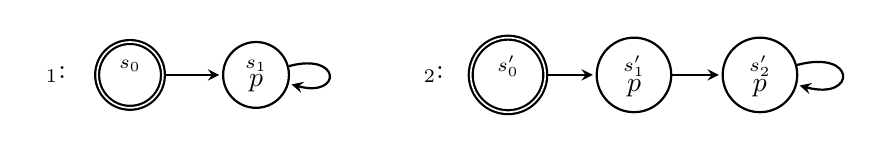
\begin{tikzpicture}[->,>=stealth,thick,shorten >=1pt,node distance=1.6cm]%,auto,node distance=2cm,every node/.style={circle,draw}]
\draw[draw=none, use as bounding box](-1.3,0.6) rectangle (9.3,-0.6);
   % \node [style={double}](v0) {$\phantom{p}$};
   % \node (v1) [right of=v0] {${p}$};
   % \draw (v0) to [right] (v1);
   % \draw (v1) to [loop right] (v1);
   % \draw [style={double}] (0,0) circle [radius=0.3];
   \node [right] at (-1.2,0) {$\Ku_1$:};
   \node [style={double,circle,draw}] (v0) {$\stackrel{s_0}{\phantom{p}}$};
   \node [style={circle,draw}, right of=v0] (v1) {$\stackrel{s_1}{p}$};
   \node [right] at (3.6,0) {$\Ku_2$:};
   \node [right of=v1] (z1) {$\phantom{p}$};
   \node [left of=v0] (z0) {$\phantom{p}$};
   \node [style={double,circle,draw}, right of=z1] (v2) {$\stackrel{s_0'}{\phantom{p}}$};
      \node [style={circle,draw}, right of=v2] (v3) {$\stackrel{s_1'}{p}$};
       \node [style={circle,draw}, right of=v3] (v4) {$\stackrel{s_2'}{p}$};
   \draw (v0) to [right] (v1);
    \draw (v1) to [loop right] (v1);
    \draw (v4) to [loop right] (v4);
    \draw (v2) to [right] (v3);
    \draw (v3) to [right] (v4);
%
\end{tikzpicture}
\caption{The finite Kripke structures $\Ku_1$ and $\Ku_2$.}\label{FigStateBasedExpressiveness}
\end{figure}

\begin{figure}[tp]
    \centering
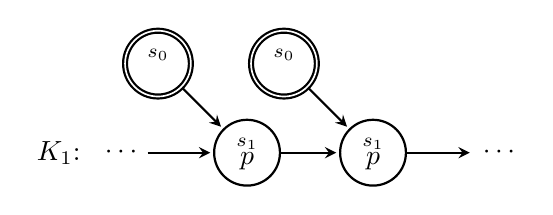
\begin{tikzpicture}[->,>=stealth,thick,shorten >=1pt,node distance=1.6cm]%,auto,node distance=2cm,every node/.style={circle,draw}]

   \node [right] at (-1.2,0) {$\mathpzc{K}_1$:};
   \node [] (v0) {$\cdots$};
   \node [style={circle,draw}, right of=v0] (v1) {$\stackrel{s_1}{p}$};
   \node [style={double,circle,draw}, above left of=v1] (v1a) {$\stackrel{s_0}{\phantom{p}}$};
   \node [style={circle,draw}, right of=v1] (v11) {$\stackrel{s_1}{p}$};
   \node [style={double,circle,draw}, above left of=v11] (v110) {$\stackrel{s_0}{\phantom{p}}$};
%   \node [style={circle,draw}, above of=v11] (v111) {$\stackrel{s_1}{p}$};
   \node [ right of=v11] (v12) {$\cdots$};
%   \node [above left of=v110] (v1x) {\Large $\ldots$};
   \draw (v0) to [right] (v1);
    \draw (v1) to (v11);
    \draw (v11) to (v12);
    \draw (v1a) to (v1);
    \draw (v110) to (v11);
%    \draw (v111) to (v11);
\end{tikzpicture}

\bigskip

\begin{tikzpicture}[->,>=stealth,thick,shorten >=1pt,node distance=1.6cm]%,auto,node distance=2cm,every node/.style={circle,draw}]
   \node [right] at (-1.2,-1) {$\mathpzc{K}_2$:};
   \node [style={double,circle,draw}] (v2) {$\stackrel{s_0'}{\phantom{p}}$};
    \node [style={circle,draw}, right of=v2] (v3) {$\stackrel{s_1'}{p}$};
    \node [style={circle,draw}, below right of=v3] (v4) {$\stackrel{s_2'}{p}$};
    \node [left of=v4] (v4x) {$\cdots$};
    \node [style={circle,draw}, right=2.5cm of v4] (v40) {$\stackrel{s_2'}{p}$};
    \node [style={circle,draw}, above left of=v40] (v401) {$\stackrel{s_1'}{p}$};
    \node [style={double,circle,draw},left of=v401] (v401x) {$\stackrel{s_0'}{\phantom{p}}$};
    \node [right of=v40] (v41) {$\cdots$};
    \draw (v2) to (v3);
    \draw (v3) to (v4);
    \draw (v3) to (v4);
    \draw (v4) to (v40);
    \draw (v40) to (v41);
    \draw (v4x) to (v4);
    \draw (v401) to (v40);
    \draw (v401x) to (v401);
\end{tikzpicture}
\caption{Forward and backward unwinding of $\mathpzc{K}_1$ and $\mathpzc{K}_2$ of Figure~\ref{FigStateBasedExpressiveness}.}\label{FigFBUnwinding}
\end{figure}

Let us consider, for instance, the two finite Kripke structures $\Ku_1$ and $\Ku_2$ of Figure~\ref{FigStateBasedExpressiveness}, whose forward and backward unwinding is shown in Figure~\ref{FigFBUnwinding}. Since $\Ku_1$ and $\Ku_2$ have the same computation tree, no $\HS$ formula $\varphi$ under the computation-tree-based semantics can distinguish $\Ku_1$ and $\Ku_2$, that is, $\Ku_1\models_\LinearPast\varphi$ if and only if $\Ku_2\models_\LinearPast\varphi$. On the other hand, the requirement ``\emph{each state reachable from the initial one where $p$ holds has a predecessor where $p$ holds as well}'' can be expressed, under the state-based semantics, by the $\HS$ formula
\[
\psi= \hsE(p\wedge \Length_1) \rightarrow \hsE(\Length_1 \wedge \hsAt(p\wedge \neg\Length_1)).
\]
It is easy to see that $\Ku_1\models_\stat\psi$: for any initial trace $\rho$ of $\Ku_1$,
we have $\Ku_1,\rho\models_\stat \hsE(p\wedge \Length_1)$ iff $\rho=s_0s_1^k$ for $k\geq 1$; the length-1 suffix $s_1$ is \emph{met-by} $s_1s_1$, and $\Ku_1,s_1s_1\models_\stat p\wedge \neg\Length_1$.
%
On the contrary, in $\Ku_2$ there is an initial trace, $s_0's_1'$, for which $\Ku_2,s_0's_1'\models_\stat\hsE(p\wedge \Length_1)$; however the only traces that meet the length-1 suffix $s_1'$ are $s_1'$ itself and $s_0's_1'$, but neither of them model $p\wedge \neg\Length_1$.
Therefore $\Ku_2\not\models_\stat\psi$. 
This allows us to prove the following proposition.

\begin{proposition}\label{Prop:StateBasedExpressiveness} 
$\HS_{\LinearPast} \not \geq \HS_\stat$.
\end{proposition}
%\begin{proof} Let us consider the two finite Kripke structures $\Ku_1$ and $\Ku_2$ of Fig.~\ref{FigStateBasedExpressiveness}. Since $\Ku_1$ and $\Ku_2$ have the same computation tree, no $\HS$ formula $\varphi$ under the computation-tree-based semantic can distinguish $\Ku_1$ and $\Ku_2$, i.e. $\Ku_1\models_\LinearPast\varphi$ iff $\Ku_2\models_\LinearPast\varphi$. We exhibit  an $\HS$ formula $\psi$ that distinguish $\Ku_1$ and $\Ku_2$ under the state-based semantics, hence, the result follows.
%\[
%\text{Let }\psi:= \langle E \rangle(p\wedge \Length_1) \rightarrow \langle E \rangle(\Length_1 \wedge \langle\overline{A}\rangle(p\wedge \neg\Length_1))
%\]
%Under the state-base semantics,  $\psi$ asserts that  each state reachable from the initial one  where $p$ holds has a predecessor where $p$ holds as well.
%Evidently, $\Ku_1\models_\stat\psi$ but $\Ku_2\not\models_\stat\psi$.
%\end{proof}

Since, as stated by  Theorem~\ref{Cor:CharacterizationHSCompTree}, $\HS_{\LinearPast}$ and finitary $\CTLStar$ have the same expressiveness and finitary $\CTLStar$ is subsumed by $\HS_\stat$ (see Corollary~\ref{cor:FromFInitaryCTLStarToFutureHSBranching}), by Proposition~\ref{Prop:StateBasedExpressiveness} the next corollary immediately follows.

\begin{corollary} $\HS_\stat$ is more expressive than $\HS_{\LinearPast}$.
\end{corollary}

In the following, we focus on the comparison of $\HS_{\LinearTime}$ with $\HS_\stat$ and $\HS_{\LinearPast}$ showing that $\HS_{\LinearTime}$ is incomparable with both $\HS_\stat$ and $\HS_{\LinearPast}$. 

The fact that  $\HS_{\LinearTime}$ does not subsume either $\HS_\stat$ or $\HS_{\LinearPast}$ can be easily proved as follows. Consider the $\CTL$ formula $\forall \Always \exists \Eventually p$ asserting that from each state reachable from the initial one, it is possible to reach a state where $p$ holds. It is well-known that this formula is not $\LTL$-definable (see~\cite{Baier2008}, Theorem~6.21). Thus, by Corollary~\ref{cor:HSLinearCharacterization}, there is no equivalent $\HS_{\LinearTime}$ formula. On the other hand, the requirement $\forall \Always \exists \Eventually p$ can be trivially expressed under the state-based (resp., computation-tree-based) semantics by the $\HS$ formula $\hsBt\hsE p $, proving the following result.

\begin{proposition}\label{prop:nonBranchingExpressibilityOfLinearTime} $\HS_{\LinearTime} \not \geq \HS_\stat$ and $\HS_{\LinearTime} \not \geq \HS_\LinearPast$.
\end{proposition}

To prove the converse, namely, that $\HS_{\LinearTime}$ is not subsumed either by $\HS_\stat$ or by $\HS_{\LinearPast}$, 
we will show that the $\LTL$ formula $\Eventually p$ (equivalent to the $\CTL$ formula $\forall \Eventually p$)
cannot be expressed in either $\HS_{\LinearPast}$ or $\HS_{\stat}$ (Proposition~\ref{prop:nonBranchingExpressibilityOfEventually}). The proof is rather involved and requires a number of definitions and intermediate results; we consider only
%We explicitly prove Proposition~\ref{prop:nonBranchingExpressibiltityOfEventually} only 
the state-based semantics, as the case of the computation-tree-based one is very similar. 

%(the result is formally stated in Proposition~\ref{prop:nonBranchingExpressibiltityOfEventually} above).


%Next we show that $\HS_{\LinearTime} \not \leq \HS_\stat$ and $\HS_{\LinearTime} \not \leq \HS_\LinearPast$.  To this end we establish the following. %is subsumed neither from $\HS_{\LinearPast}$ nor from $\HS_{\stat}$, we establish the following  result.

Let us start by defining two families of Kripke structures $(\Ku_n)_{n\geq 1}$ and $(\mathpzc{M}_n)_{n\geq 1}$ over $\{p\}$ such that for all $n\geq 1$, the $\LTL$ formula $\Eventually p$
 distinguishes $\Ku_n$ and  $\mathpzc{M}_n$, and for every $\HS$ formula $\psi$ of size at most $n$, $\psi$ does \emph{not} distinguish
 $\Ku_n$ and  $\mathpzc{M}_n$ under the state-based semantics. 
 %Hence the result follows.
 
For a given $n \geq 1$, the Kripke structures $\Ku_n$ and $\mathpzc{M}_n$ are depicted in
 Figure~\ref{FigEventuallyNOnBranchingExpressible}. Notice that the Kripke structure $\mathpzc{M}_n$  differs from  $\Ku_n$ only in that its initial state is $s_1$ instead of $s_0$. Formally, $\Ku_n=(\{p\},\States_n, \Edges_n,\Lab_n,s_0)$ and $\mathpzc{M}_n=(\{p\},\States_n, \Edges_n,\Lab_n,s_1)$, with
 $\States_n=\{s_0,s_1,\ldots, s_{2n},t\}$, $\Edges_n=\{(s_0,s_0),(s_0,s_1),\ldots, (s_{2n-1},s_{2n}),\allowbreak (s_{2n},t),(t,t)\}$,  $\Lab(s_i)=\emptyset$ for all $0\leq i\leq 2n$, and $\Lab(t)=\{p\}$. 
 
It is immediate to see that
%
 %\begin{remark}\label{FirstRemarkEventuallyNOnBranchingExpressibl%e} 
 $\Ku_n\not\models \Eventually p$ and $\mathpzc{M}_n\models \Eventually p$.
 %\end{remark}

\begin{figure}[t]%[5]{l}{1\linewidth}
\centering
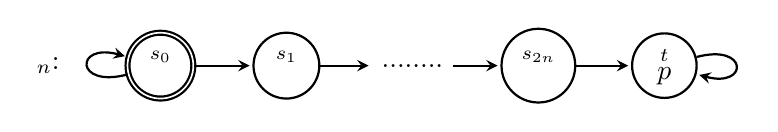
\begin{tikzpicture}[->,>=stealth,thick,shorten >=1pt,node distance=1.6cm]%,auto,node distance=2cm,every node/.style={circle,draw}]
   % \node [style={double}](v0) {$\phantom{p}$};
   % \node (v1) [right of=v0] {${p}$};
   % \draw (v0) to [right] (v1);
   % \draw (v1) to [loop right] (v1);
   % \draw [style={double}] (0,0) circle [radius=0.3];
   \node [right] at (-1.7,0) {$\Ku_n$:};
   \node [style={double,circle,draw}] (v0) {$\stackrel{s_0}{\phantom{p}}$};
%   \node [right] at (-0.3,-0.6) {$s_0$};
%   \node [right] at (1.3,-0.6) {$s_1$};
%   \node [right] at (4.5,-0.6) {$s_{2n}$};
%   \node [right] at (6.1,-0.6) {$t$};
   \node [style={circle,draw}, right of=v0] (v1) {$\stackrel{s_1}{\phantom{p}}$};
   \draw (v0) to [right] (v1);
       \draw (v0) to [loop left] (v0);
   \node [right of=v1] (v2) {$........$};
   \draw (v1) to [right] (v2);
   \node [style={circle,draw},right of=v2] (v2n) {$\stackrel{s_{2n}}{\phantom{p}}$};
   \draw (v2) to [right] (v2n);
   \node [style={circle,draw}, right of=v2n] (v) {$\stackrel{t}{p}$};
      \draw (v) to [loop right] (v);
   \draw (v2n) to [right] (v);
\end{tikzpicture}

\bigskip

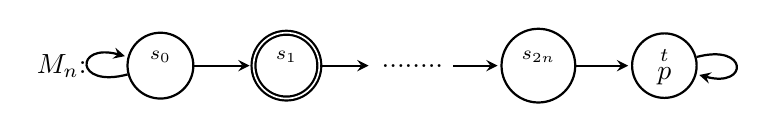
\begin{tikzpicture}[->,>=stealth,thick,shorten >=1pt,node distance=1.6cm]%,auto,node distance=2cm,every node/.style={circle,draw}]
   % \node [style={double}](v0) {$\phantom{p}$};
   % \node (v1) [right of=v0] {${p}$};
   % \draw (v0) to [right] (v1);
   % \draw (v1) to [loop right] (v1);
   % \draw [style={double}] (0,0) circle [radius=0.3];
   \node [right] at (-1.7,0) {$\mathpzc{M}_n$:};
   \node [style={circle,draw}] (v0) {$\stackrel{s_0}{\phantom{p}}$};
%   \node [right] at (-0.3,-0.6) {$s_0$};
%   \node [right] at (1.3,-0.6) {$s_1$};
%   \node [right] at (4.5,-0.6) {$s_{2n}$};
%   \node [right] at (6.1,-0.6) {$t$};
   \node [style={double,circle,draw}, right of=v0] (v1) {$\stackrel{s_1}{\phantom{p}}$};
   \draw (v0) to [right] (v1);
       \draw (v0) to [loop left] (v0);
   \node [right of=v1] (v2) {$........$};
   \draw (v1) to [right] (v2);
   \node [style={circle,draw},right of=v2] (v2n) {$\stackrel{s_{2n}}{\phantom{p}}$};
   \draw (v2) to [right] (v2n);
   \node [style={circle,draw}, right of=v2n] (v) {$\stackrel{t}{p}$};
      \draw (v) to [loop right] (v);
   \draw (v2n) to [right] (v);
\end{tikzpicture}
\caption{The finite Kripke structures $\Ku_n$ and $\mathpzc{M}_n$ with $n\geq 1$.}\label{FigEventuallyNOnBranchingExpressible}
\end{figure}

On the contrary, with the next Lemma~\ref{lemma:MainnonBranchingExpressibilityOfEventually}, we are going to prove that  $\Ku_n\models_\stat \psi$ if and only if $\mathpzc{M}_n\models_\stat \psi$ for all balanced $\HS_\stat$ formulas $\psi$ of length at most $n$, with $n\geq 1$. 
An $\HS_\stat$ formula $\psi$ is \emph{balanced} if, for each subformula $\hsB \theta $ (resp., $\hsBt \theta $), $\theta$ has the form $\theta_1\wedge\theta_2$ with $|\theta_1| = |\theta_2|$. Proving the result for  balanced $\HS_\stat$ formulas allows us to state it for any $\HS_\stat$ formula, since it is possible to trivially 
convert an $\HS_\stat$ formula $\psi$ into a balanced one (by using conjunctions of $\top$) which is equivalent to $\psi$ under any of the considered $\HS$ semantic variants.

\begin{lemma}\label{lemma:MainnonBranchingExpressibilityOfEventually} For all $n\in\Nat^+$ and balanced $\HS_\stat$ formulas $\psi$, with $|\psi|\leq n$, 
it holds that $\Ku_n\models_\stat \psi$ if and only if $\mathpzc{M}_n\models_\stat \psi$.
\end{lemma}
The complete proof is in Appendix~\ref{proof:lemma:MainnonBranchingExpressibilityOfEventually}.

As an immediate consequence of Lemma~\ref{lemma:MainnonBranchingExpressibilityOfEventually} and of the fact that, for each $n\geq 1$,  $\Ku_n\not\models \Eventually p$ and $\mathpzc{M}_n\models \Eventually p$, we get the desired undefinability result.
%get a proof of Proposition~\ref{prop:nonBranchingExpressibiltityOfEventually}.

%\begin{lemma}\label{lemma:MainnonBranchingExpressibiltityOfEventually} Let $n\geq 1$ and $\psi$ be a balanced $\HS$ formula such that $|\psi|\leq n$.
%Then, $\Ku_n\models_\stat \psi$ iff $\mathpzc{M}_n\models_\stat \psi$.
%\end{lemma}

%The proof of Lemma~\ref{lemma:MainnonBranchingExpressibiltityOfEventually} is concluded.

%deduce the following corollary which, together with Property~\ref{remark:HcompatibilityTwo}, finally provides a proof of
%Lemma~\ref{lemma:MainnonBranchingExpressibiltityOfEventually} (recall that $\Ku_n$ and $\mathpzc{M}_n$ differ only in the initial state, which is $s_0$ for $\Ku_n$ and $s_1$ for $\mathpzc{M}_n$).

\begin{proposition}\label{prop:nonBranchingExpressibilityOfEventually} 
The $\LTL$ formula $\Eventually p$ (equivalent to the $\CTL$ formula $\forall \Eventually p$) cannot be expressed in either $\HS_{\LinearPast}$ or $\HS_{\stat}$.
\end{proposition}

The next proposition follows from Corollary \ref{cor:HSLinearCharacterization} and Proposition~\ref{prop:nonBranchingExpressibilityOfEventually}.

\begin{proposition}\label{prop:oppositeDirection} $\HS_\stat \not \geq  \HS_{\LinearTime} $ and $\HS_\LinearPast \not \geq \HS_{\LinearTime}$.
\end{proposition}

Putting together Proposition~\ref{prop:nonBranchingExpressibilityOfLinearTime} and Proposition~\ref{prop:oppositeDirection}, we finally obtain the incomparability result.

\begin{theorem} 
$\HS_\LinearTime$ and $\HS_\stat$  are expressively incomparable, and so are $\HS_\LinearTime$ and $\HS_\LinearPast$.
\end{theorem}

The proved results also allow us to establish  the  expressiveness relations between  $\HS_\stat$, $\HS_\LinearPast$ and the standard branching temporal logics $\CTL$ and $\CTLStar$.

%\subsection{Expressiveness comparison between  $\HS_\stat$ (resp., $\HS_\LinearPast$) and standard temporal logics}

\begin{corollary}
The following expressiveness results hold:
\begin{enumerate}
\item $\HS_\stat$ and $\CTLStar$ are expressively incomparable;
\item $\HS_\stat$ and $\CTL$ are expressively incomparable;
\item $\HS_\LinearPast$ and finitary $\CTLStar$ are  less expressive than $\CTLStar$;
\item  $\HS_\LinearPast$ and $\CTL$ are expressively incomparable.
\end{enumerate}
\end{corollary}
\begin{proof}
\begin{enumerate}
\item By Proposition~\ref{prop:nonBranchingExpressibilityOfEventually} and the fact that  $\CTLStar$ is not sensitive to unwinding. %, the results follows from Proposition~\ref{Prop:StateBasedExpressiveness}
%and Proposition~\ref{prop:nonBranchingExpressibiltityOfEventually}.

\item Again, by Proposition~\ref{prop:nonBranchingExpressibilityOfEventually} and by the observation that $\CTL$ is not sensitive to unwinding.

\item By Theorem~\ref{Cor:CharacterizationHSCompTree},  $\HS_\LinearPast$ is subsumed by $\CTLStar$, and $\HS_\LinearPast$ and finitary $\CTLStar$ have the same expressiveness. %The inclusions are strict by
Hence, by Proposition~\ref{prop:nonBranchingExpressibilityOfEventually}, the result follows.

\item Thanks to Proposition~\ref{prop:nonBranchingExpressibilityOfEventually}, it suffices to show that there exists a
$\HS_\LinearPast$ formula which cannot be expressed in $\CTL$. 

Let us consider the $\CTLStar$ formula
$\varphi= \EQ\bigl(((p_1 \until p_2) \vee (q_1 \until q_2)) \until r\bigr)$
over the set of propositions $\{p_1,p_2,q_1,q_2,r\}$. It is shown in~\cite{EH86} that $\varphi$
cannot be expressed in $\CTL$. Clearly, if
we replace the path quantifier $\EQ$ in $\varphi$ with the finitary path quantifier $\EQF$,  we obtain an equivalent formula of finitary $\CTLStar$.
Thus, since $\HS_\LinearPast$ and finitary $\CTLStar$ have the same expressiveness (Theorem~\ref{Cor:CharacterizationHSCompTree}),
the result follows.\qedhere
\end{enumerate}
\end{proof}


% \begin{corollary} $\HS_\stat$ and $\CTLStar$ (resp., $\CTL$) are expressively incomparable.
% \end{corollary}

% Moreover, since $\HS_\LinearPast$ is subsumed by $\CTLStar$, and $\HS_\LinearPast$ and finitary $\CTLStar$ have the same expressiveness (Corollary~\ref{Cor:CharacterizationHSCompTree}), by Proposition~\ref{prop:nonBranchingExpressibiltityOfEventually},
% the following holds.

% \begin{corollary} $\HS_\LinearPast$ and finitary $\CTLStar$ are  less expressive than $\CTLStar$.
% \end{corollary}
%Lastly, we observe the following.

% \begin{corollary} $\HS_\LinearPast$ and $\CTL$ are expressively incomparable.
% \end{corollary}
% \begin{proof}
% By Proposition~\ref{prop:nonBranchingExpressibiltityOfEventually}, it suffices to show that there is a
% $\HS_\LinearPast$ formula which cannot be expressed in $\CTL$. Let us consider the $\CTLStar$ formula
% $\varphi:= \EQ\bigl(((p_1 \until p_2) \vee (q_1 \until q_2)) \until r\bigr)$
% over the set of propositions $\{p_1,p_2,q_1,q_2,r\}$. It is shown in \cite{emerson1986sometimes} that the above $\CTLStar$ formula
% cannot be expressed in $\CTL$. Evidently, if
% we replace the path quantifier $\EQ$ in $\varphi$ with the finitary path quantifier $\EQF$,  we obtain an equivalent formula of finitary $\CTLStar$.
% Thus, since $\HS_\LinearPast$ and finitary $\CTLStar$ have the same expressiveness (Corollary~\ref{Cor:CharacterizationHSCompTree}),
% the result follows.
% \end{proof}

